Inicialmente, foram analisadas as propostas para o fornecimento energético do Sistema Integrado de Monitoramento, foram elas, eólica, solar, e também a possibilidade do sistema ser ligado à rede concessionária, ou seja, um sistema \textit{on grid}.
A tomada de decisão, levou em conta fatores relevantes e que pudessem afetar o bom desempenho do equipamento foram postos em pauta, e devidamente justificados no Ponto de Controle 01 (PC01). Com base nos pontos positivos e negativos analisados de cada proposta, a escolha que apresentou maior viabilidade para agregar ao projeto foi o sistema ligado na rede, assim como a proposta que atende a maioria das casas no Brasil.
O fornecimento energético do SUM, será feito semelhante à uma residência normal, como mostrado no esquemático abaixo.

Como demonstrado, a energia elétrica chegará no QGBT (Quadro Geral de Baixa Tensão), semelhante aos presentes em construções civis, em seguida, serão feitas as devidas distribuições, de acordo com a demanda para as estruturas do SUM.

\begin{figure}[H]
	\centering
	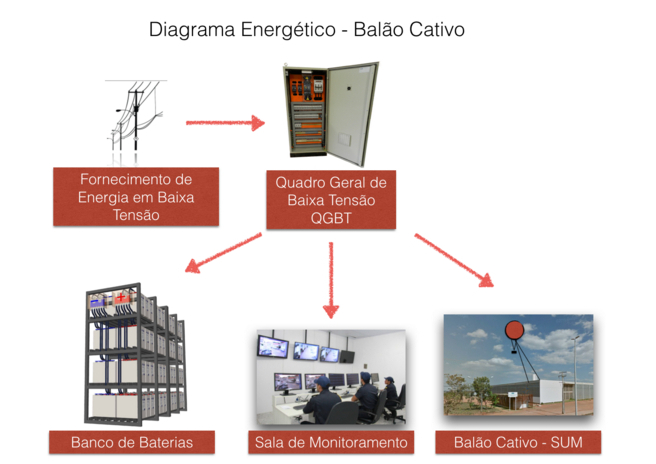
\includegraphics[width=0.6\textwidth]{figuras/Energetico}
	\caption{Diagrama Energético - Balão Cativo.}
	\label{img:Energetico}
\end{figure}

 \subsection{QGBT (Quadro Geral de Baixa Tensão):}
 Painéis que acomodam o equipamentos para a proteção, seccionamento e manobra de energia elétrica. Os painéis podem variar de tamanho, desde residenciais até painéis de grandes de indústrias, edificações comerciais, hospitais, entre outros. O dimensionamento do QGBT é de grande importância para manter a integridade e a segurança de todo o sistema.

\subsection{Banco de Baterias:}

As baterias elétricas têm sido utilizadas principalmente voltada a elementos acumuladores em sistemas de alimenta\c{c}ão ininterruptos. O banco de baterias é o conjunto delas ligados em paralelo ou série-paralelo, visando atender à necessidade do sistema em situações emergenciais. O dimensionamento correto do banco de baterias irá garantir a continuidade das operações do sistema por um determinado período de tempo.

\begin{figure}[H]
	\centering
	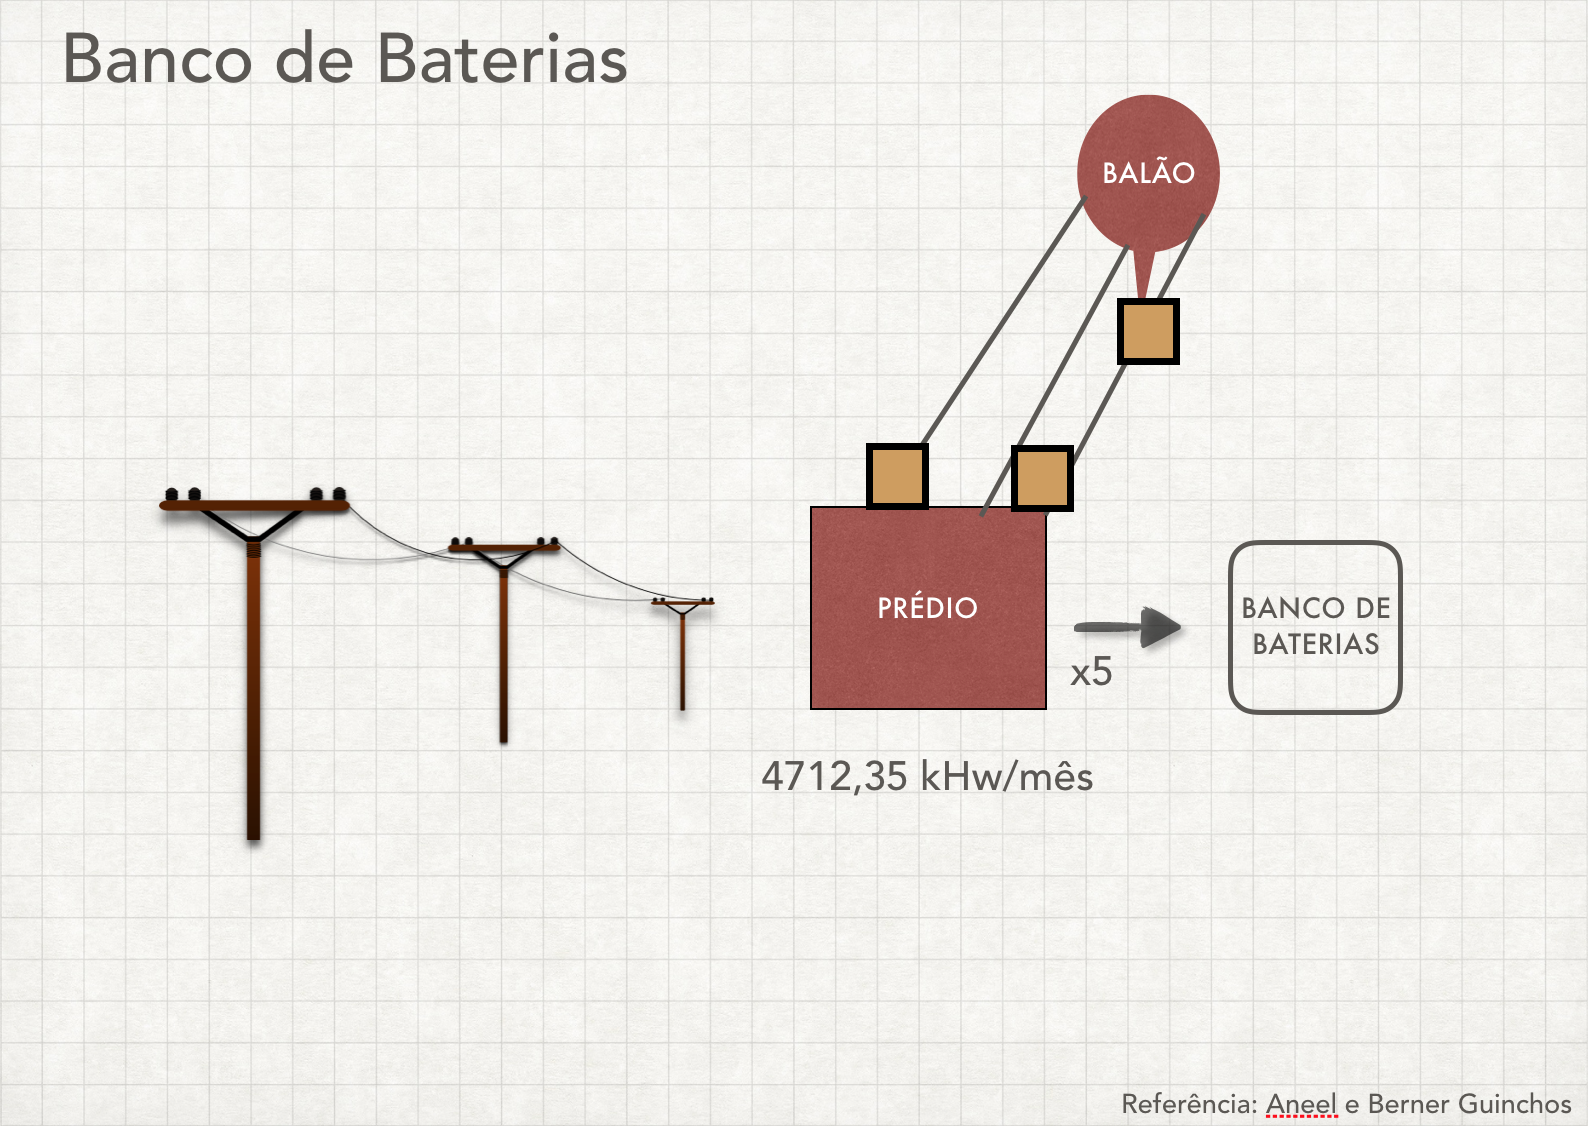
\includegraphics[width=0.6\textwidth]{figuras/baterias}
	\caption{Banco de Baterias.}
	\label{img:baterias}
\end{figure}

\subsubsection{Dimensionamento do Banco de Baterias:}

Funciona como um sistema emergencial, quando a energia fornecida pela rede falha, ou não é o suficiente para o bom funcionamento do conjunto. O objetivo é manter funcionando apenas as estruturas vitais, para que a segurança não seja prejudicada. No caso, manteremos apenas os monitores, um computador, e a estrutura do balão, resultando num consumo de 2015,55 kWh, para ser suprido pelas baterias por um período máximo de 6 horas de autonomia.
Com auxílio da calculadora Digitek, baterias semelhante às automotivas, com 12 Volts e 70 ampéres, um inversor com eficiência próxima de 80\%, conseguimos a seguinte disposição:

\begin{figure}[H]
	\centering
	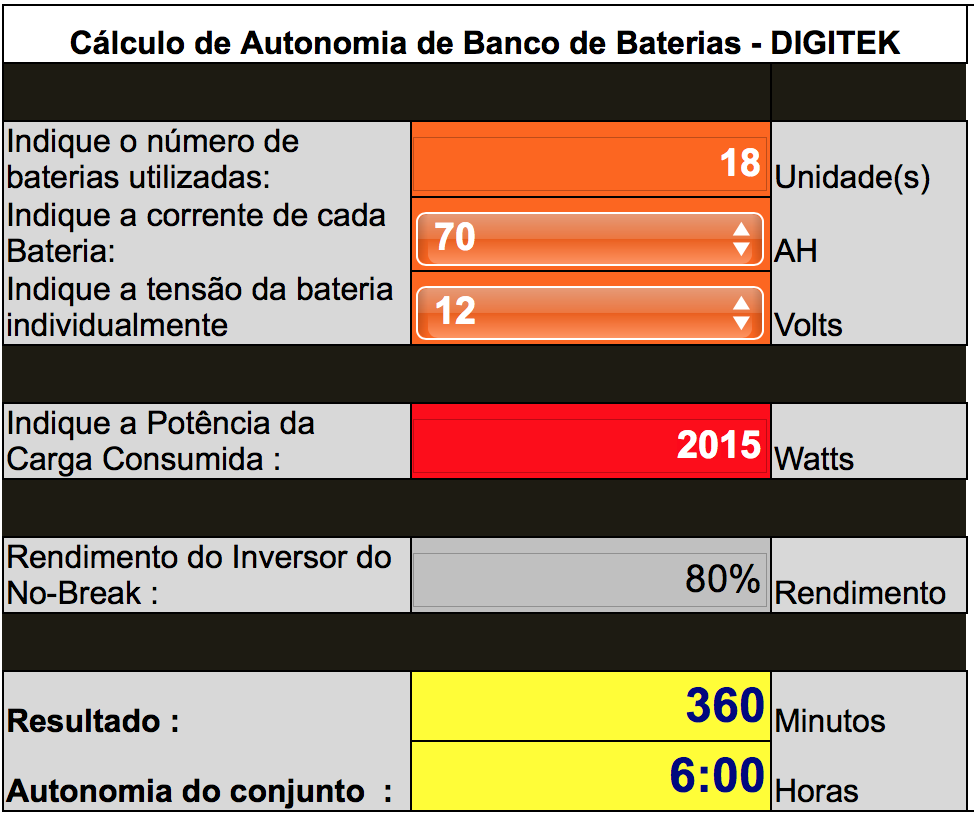
\includegraphics[width=0.6\textwidth]{figuras/calculo}
	\caption[Cálculo de autonomia de Banco de baterias]{Cálculo de autonomia de Banco de baterias~\cite{digitek}}
	\label{img:calculo}
\end{figure}


Um banco de 18 unidades de bateria de chumbo (Pb), 12 Volts e 70A, ligadas em paralelo, vão atender à necessidade do sistema por um período de 6 horas.
Em face do exposto, e fazendo uma breve análise do que foi apresentado, temos todas as estruturas que consumirão energia dispostas em forma de esquemáticos indicando seus respectivos consumos, dimensionamento dos fios de acordo com a NBR 5410 da ABNT, dimensionamento do banco de bateria para situações emergenciais e análise do quanto será demandado de energia para o funcionamento completo do SUM.

\subsection{Elementos consumidores do SUM}

Abaixo, temos um resumo esquemático simplificado das estruturas que são as potenciais consumidoras do conjunto, sendo assim, utilizadas como base de cálculo para o dimensionamento do banco de baterias, e dos fios de transmissão.
	Para isso, separamos em dois blocos independentes, a Sala de Monitoramento (SM) e o Sistema do Balão (SB)  para o desenvolvimento dos cálculos, considerando o fornecimento da Companhia Energética de Brasília (CEB), com 220 Volts, 60Hz. (CEB, 2002)
	O cálculo do consumo mensal de cada equipamento, tanto da sala de monitoramento quanto do sistema do balão, foi dado pelo produto da potência do equipamento em watt, pela quantidade de horas que ele é utilizado ao dia e o número de dias do mês, isso sendo dividido por 1000. Os equipamentos serão utilizados 24h por dia, e para a realização dos cálculos, o mês foi considerado de 30 dias.
Quando feito o somatório dos valores do consumo mensal de cada equipamento, é obtido o consumo mensal da sala de monitoramento e também o consumo mensal do sistema do balão.

Consumo total =  $\sum ((Potência do equipamento(w) x 24h x 30 dias)/1000)$ %

 \subsubsection{Sala de Monitoramento:}

 A sala de monitoramento, apresenta em seu âmbito os equipamentos de observação e processamento dos dados, como monitores, backup, com funcionamento ininterrupto, já que estamos tratando de um sistema de segurança, operando na vigência 24/7.
Como podemos imaginar, a sala de monitoramento será a maior consumidora de energia do conjunto, por apresentar dispositivos que tornem o ambiente favorável ao trabalho de monitoramento, como: monitores, iluminação, temperatura adequada para operação dos equipamentos, entre outros equipamentos auxiliares. O dimensionamento da sala de deve levar em conta as necessidades mínimas para que em situações emergenciais o sistema continue operando sem prejuízos.
A Sala de Monitoramento, apresenta dois monitores Samsung 42’’, dois computadores de alta performance, um aparelho de ar condicionado LG de 12.000 BTUs, e oito luminárias tubulares de LED (\textit{Light Emission Diode}).



Segue abaixo um esquemático com os resultados dos cálculos do consumo energético dos equipamentos, e da sala:

\begin{figure}[H]
	\centering
	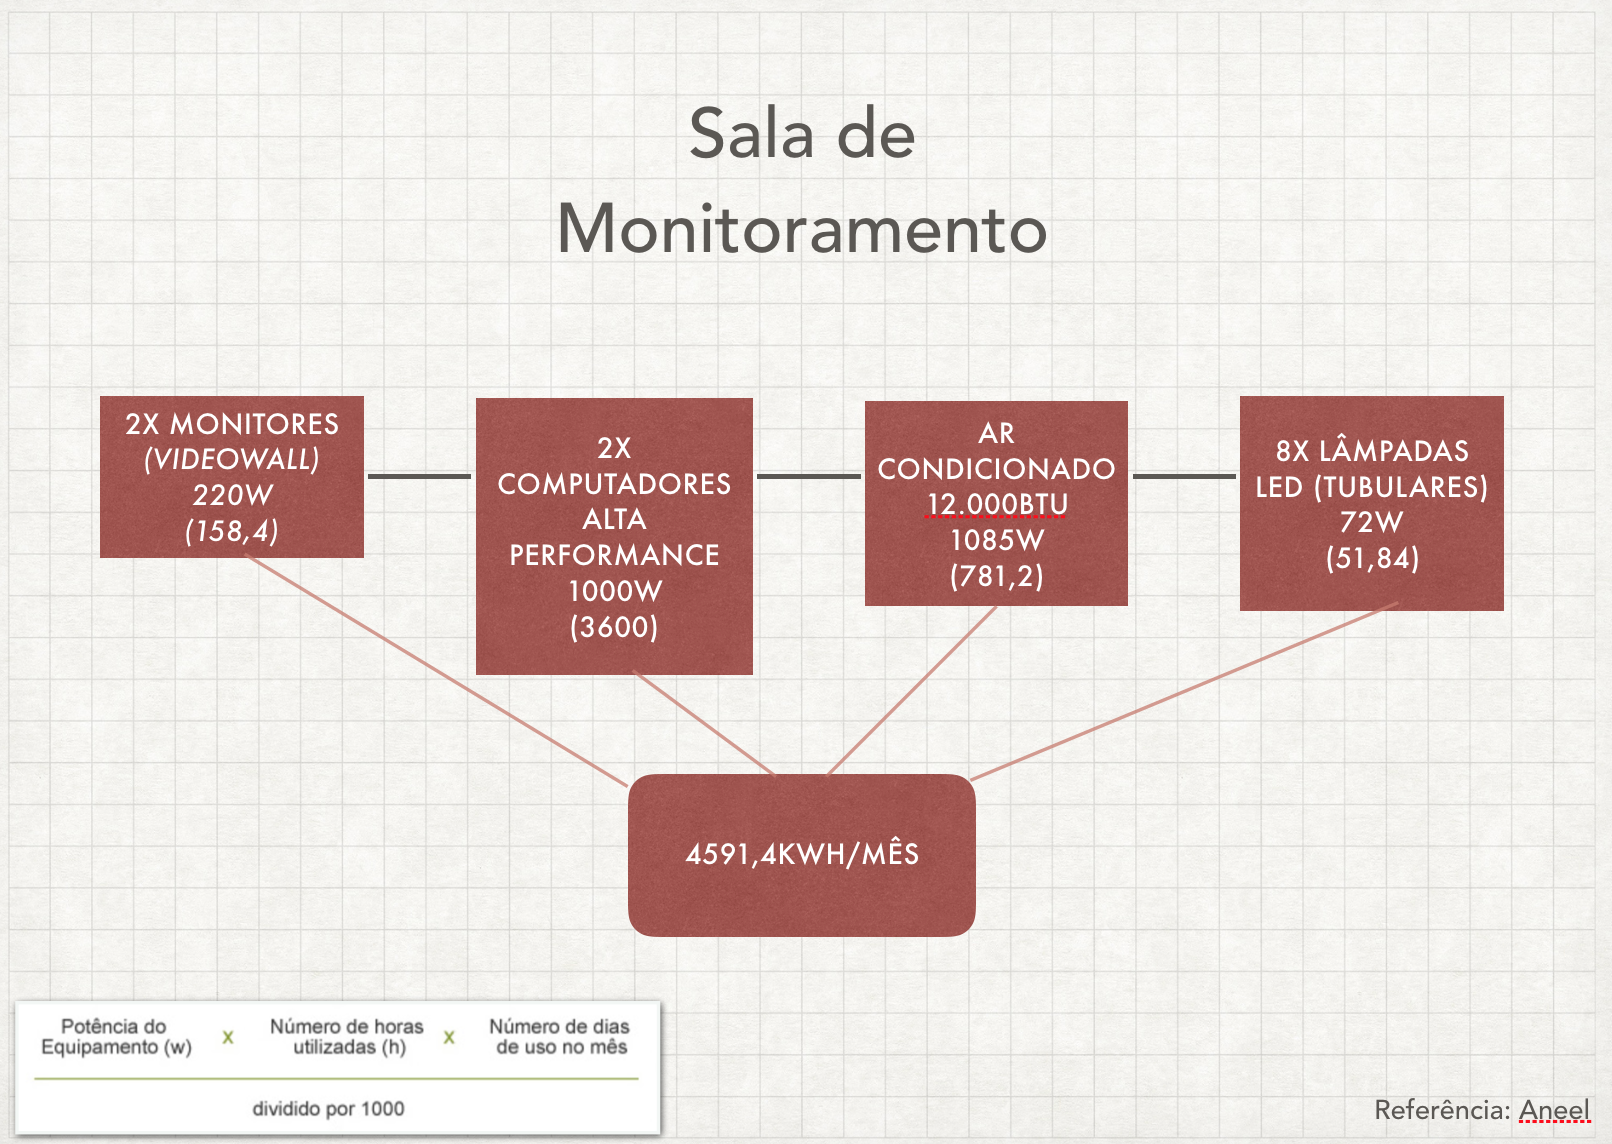
\includegraphics[width=0.6\textwidth]{figuras/salaMonitoramento}
	\caption{Sala de monitoramento}
	\label{img:salaMonitoramento}
\end{figure}


\subsubsection{Sistema do Balão}

O Sistema do Balão, apresenta menor consumo, e também menos itens, temos a payload, composta por sensores, eletrônica e as câmeras, e também o sistema de guinchos, utilizados no recolhimento do balão.
Segue abaixo um esquemático com os resultados dos cálculos do consumo energético dos equipamentos, e do sistema:

\begin{figure}[H]
	\centering
	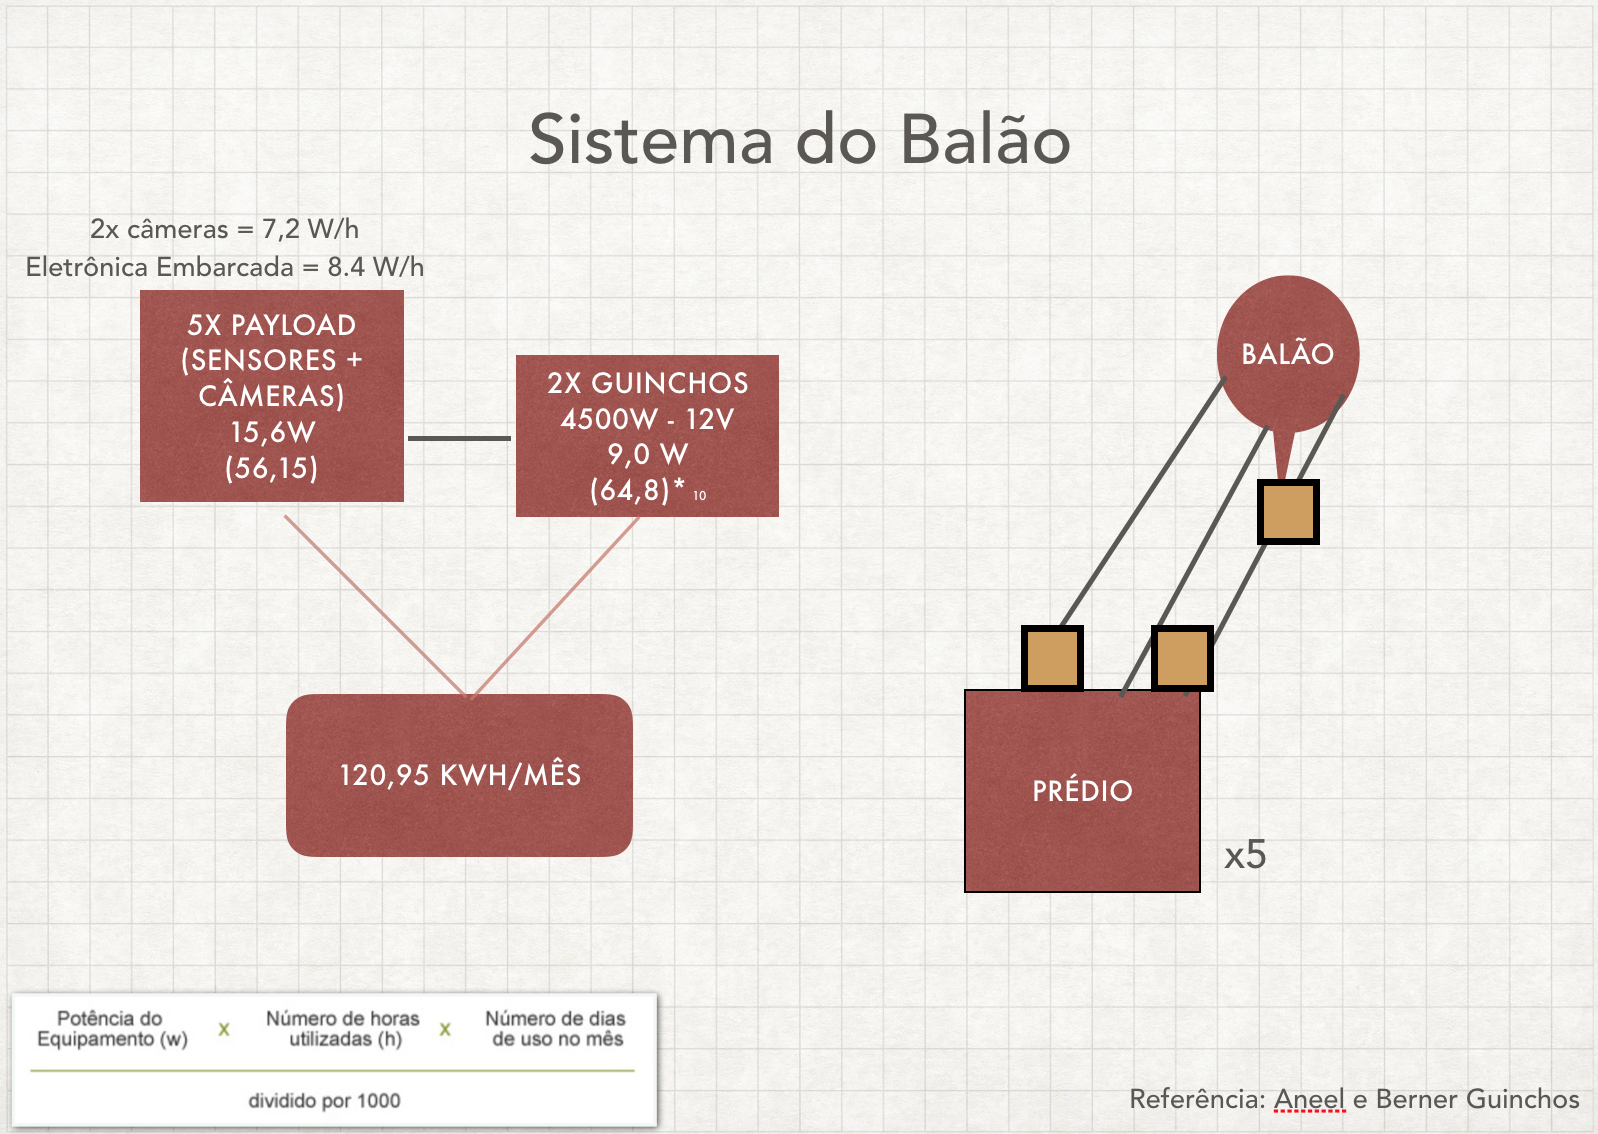
\includegraphics[width=0.6\textwidth]{figuras/sistemaBalao}
	\caption{Sistema do balão}
	\label{img:sistemaBalao}
\end{figure}


Para a determinação da espessura dos fios, utilizamos a Norma Brasileira de Regulamentação 5410/2004, referente a instalações elétricas de baixa tensão. Conforme a tabela abaixo, para as estruturas luminosas, serão utilizados fio de 1,5mm de espessura, para as tomadas de energia e dispositivos para conectar os equipamentos na Sala de Monitoramento, serão utilizados fios de 2,5mm de espessura. Para a alimentação do balão, por ser uma estrutura de baixa demanda energética, será utilizado um fio de 0,5mm de espessura, conforme determina a NBR.

\begin{figure}[H]
	\centering
	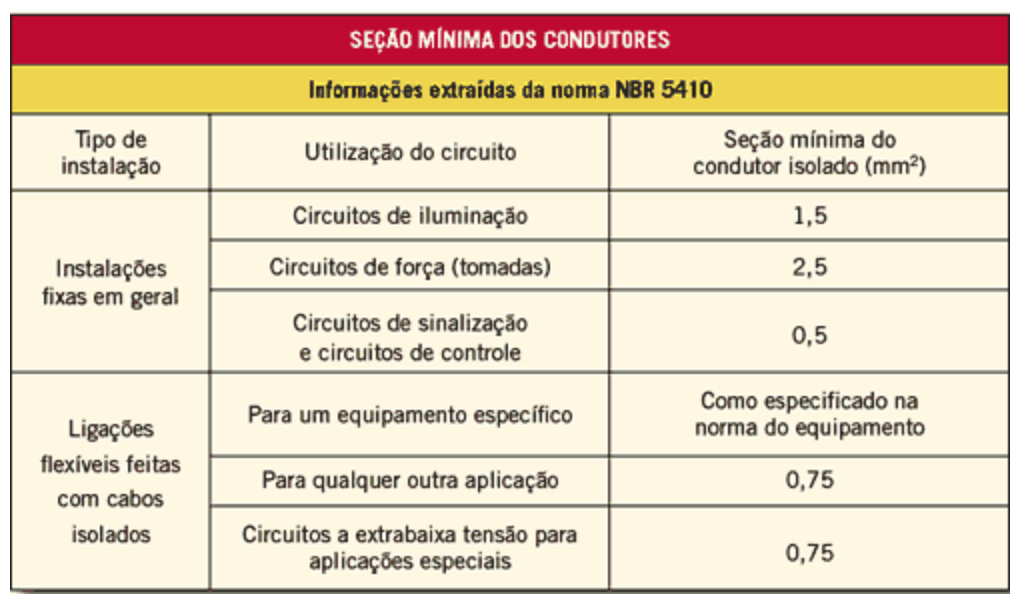
\includegraphics[width=0.6\textwidth]{figuras/BitoladoFio}
	\caption{Bitola do Fio}
	\label{img:BitoladoFio}
\end{figure}
